This section covers how we chose to handle the prediction requirement.

\subsection{Gathering statistical data}
\label{ssub:statisticaldata}
Storing data about past activity in a room can be done in a variety of ways. In our final design we chose to store data about how occupied each section of the recorded image is in addition to just storing data about each occupant. The process is simple; we split the image of a room into sections, referred to as cells, and each time an occupant enters a cell the stored activity value for the given cell is increased. This value starts at 1 and grows towards infinity. Each room has a different and independent set of cells. This activity data tells us which sections of the room are most occupied. We use the activity data to calculate probabilities about an occupant's future possible actions using our own custom prediction model, explained in the following section.

\subsection{Custom prediction model based on HMM}
\label{ssub:designcustomprediction}
We have chosen to build our own prediction model heavily inspired by the hidden Markov model. Each cell in the image is a state where the state transition probability is the likelihood of an occupant moving to an adjacent cell and the output probability is the likelihood of an occupant going to an exit given any current cell. Unlike a regular hidden Markov model, we do not store probability values individually for each state, because each probability is dependant upon several factors that differ from each occupant. Instead, we do the necessary calculations each time a prediction is requested by using the stored activity values of each cell. As mentioned in the previous section, the activity value describes how occupied a cell has been and functions like a base weight when calculating the probabilities. Our custom model modifies this weight or value by taking several custom factors into account during calculations. These factors work as a rule set for likely or unlikely occupant actions and have an impact on the probabilities:
\begin{enumerate}
\item An occupant entering a room from a given exit is less likely to exit the room at the given exit.
\item An occupant is more likely to continue moving in his general direction, less likely to change direction and least likely to return to his previously visited cell.
\item An occupant is more likely to move to the adjacent cell with the highest amount of previous activity.
\item The likelihood of an occupant exiting at a given exit (unless it also serves as the occupant's entrance) is inversely proportional to the direct distance to the given exit, producing a magnet-like effect.
\end{enumerate}
Item 1 is handled by inferring an occupant's entrance cell by looking at the occupant's first coordinate in the stored path. During calculations, the value of an entrance cell is significantly lowered by a modifier. Item 2 is handled by inferring an occupant's previously visited cell by scanning the path from the end until a coordinate residing in a different cell is found. The value of this cell is significantly lowered by a modifier while the value of the cell on the direct opposite side of the current cell is raised by another modifier. Item 3 is supported by the adjacent cell with the most activity simply having a greater base value. Item 4 is supported by using the following function to modify the value of a cell: \\
\begin{equation}
v = \frac{v}{k^d}
\end{equation}
\\
where \(v\) is the value of a cell, \(k\) is some constant and \(d\) is the distance in some unit. \\
Adjusting \(k\) will increase or decrease the impact the distance has on the value. The higher \(d\) is, the lower \(v\) becomes. Using the modifiers, all of these factors have a significant influence on the final value or weight of a cell or exit, which is used when calculating each probability. The higher the value, the greater probability. The sum of the probabilities of an occupant moving to each individual exit or each adjacent cell given a current cell is 1. The cell with the highest probability will be the predicted cell.
\begin{figure}[htb]
\centering
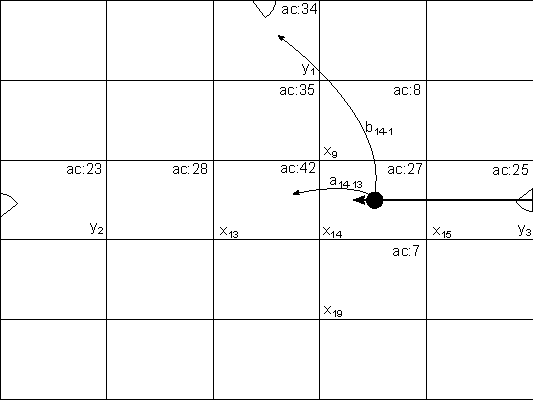
\includegraphics{prediction_figures/custom}
\caption{Applying the custom model to a scenario.}
\label{fig:custom_model}
\end{figure}

Figure \ref{fig:custom_model} shows the custom model translated to a scenario. Each cell contains an identification number, an activity count and a value denoting whether or not the cell is an exit cell. The occupant entered the room at exit \(y_3\) and the current state is \(x_{14}\). \(a_{14-13}\) denotes the state transition probability of the occupant moving from state \(x_{14}\) to state \(x_{13}\). \(b_{14-1}\) denotes the output probability of the occupant ultimately choosing exit \(y_{1}\). Taking our custom rule set into account, the occupant is least likely to exit at \(y_3\) and most likely to continue to \(x_{13}\). Moving to \(x_9\) would increase the probability of the occupant exiting at \(y_{1}\) (\(b_{9-1}\)) significantly.